% 页面设置
\documentclass[12pt, a4paper]{article} % 字号:12,纸张:A4
\usepackage[top=2.54cm, bottom=2.54cm, left=3.18cm,right=3.18cm]{geometry} % 页边距设置
% 字体设置
\usepackage[UTF8]{ctex}
\usepackage{fontspec} % 设置字体
%\setCJKmainfont{SimSun}[AutoFakeBold=true, BoldFont={SimHei}, ItalicFont={KaiTi}] % 正文字体
%\setCJKsansfont[AutoFakeBold=3]{KaiTi} % 无衬线字体
%\setCJKmonofont[AutoFakeBold=3]{SimHei} % 等宽字体
\setmainfont{Times New Roman} % 设置主字体为新罗马体
% 文本设置
\usepackage{enumerate} % 支持小标题编号
\linespread{1.5} % 行间距1.5倍
\usepackage{indentfirst}%首段缩进
\setlength{\parindent}{2em} % 首行缩进两字符
\usepackage[hidelinks]{hyperref} % 目录添加超链接
\usepackage{zhnumber} % 章节标题中文显示
\usepackage[cmyk]{xcolor} % 文字彩色显示
% 数学支持
\usepackage{amsmath} % 数学公式支持
\usepackage{amssymb} % 数学符号支持
\usepackage{bm} % 公式加粗
\usepackage{mathrsfs} % 花体字母
\usepackage{yhmath} % 更多的数学符号
% 图片设置
\usepackage{caption} % 插入图片标题
\usepackage{float} % 控制图片位置
\usepackage{subfigure} % 图片并排
\usepackage{booktabs} % 插入表格
% 表格设置
\usepackage{multirow} % 表格自动换行
\usepackage{bigstrut} % 表格间距
\usepackage{rotating} % 表格旋转
\usepackage{tabularx} % 表格宽度
\usepackage{colortbl} % 表格颜色
\usepackage{graphicx} % 表格自动宽度

\title{第八章 \ \ \ 集成学习} % 文章标题
\author{Castor Ye} % 文章作者
\date{} % 文章时间

\begin{document} % 文档从这里开始。
\maketitle % 按照预定的模板把上面那些信息排好。
\newtheorem{definition}{定义}[section]
\newtheorem{theorem}{定理}[section]
\newtheorem{example}{例}[section]
\newtheorem{solution}{题解}
\newtheorem{algorithm}{算法}
\newtheorem{axiom}{公理}
\newtheorem{property}{性质}
\newtheorem{proposition}{命题}
\newtheorem{lemma}{引理}
\newtheorem{corollary}{推论}[section]
\newtheorem{remark}{注解}
\newtheorem{condition}{条件}
\newtheorem{conclusion}{结论}
\newtheorem{assumption}{假设}
\renewcommand{\figurename}{图} % 将图片序号改为图
\renewcommand{\tablename}{表} % 将表格序号改为表
%%%%%%%%%%%%%%%%%%%%%%%%%%%%%%%%%%%%%%%%%%%%%%%%%%%%%%%%%%%%%%%%%%%%%%%
% 文章内容从此开始
\section{个体与集成}

集成学习(ensemble learning)通过构建并结合多个学习器来完成学习任务,有时也被称为多分类器系统(multi-classfier system)、基于委员会的学习(committee-based learning)等。

图 \ref{fig:集成学习示意图} 显示出集成学习的一般结构:先产生一组“个体学习器”(in地vi learner),再用某种策略将它们结合起来。

\begin{figure}[H]
    \centering
    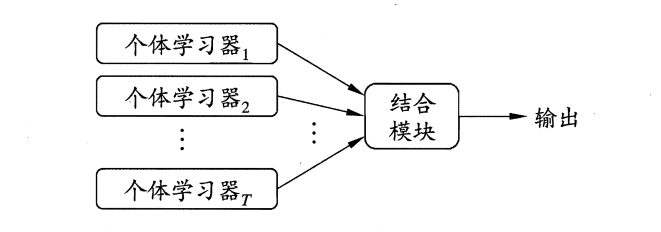
\includegraphics[width=0.8\textwidth]{../img/8-1-集成学习示意图.png}
    \caption{集成学习示意图}
    \label{fig:集成学习示意图}
\end{figure}

在集成模型中,若个体学习器都属于同一类别,例如都是决策树或神经网络,则称该集成为“同质”的(homogenneous)。同质集成中的个体学习器亦称“基学习器”(base learner),相应的学习算法称为“基学习算法”(base learning algorithm)。若个体学习器为不同类型的,则称该集成为“异质”的(heterogenous)。异质集成中的个体学习器由不同的学习算法生成,此时不再有基学习器,而称“组件学习器”(component learner)或直接称“个体学习器”。

上面我们已经提到要让集成起来的泛化性能比单个学习器好,但也存在短板效应,所以我们引入两个重要概念:准确性和多样性(diversity)。准确性指的是个体学习器不能太差,要有一定的准确度;多样性则是个体学习器之间的输出要具有差异性。

\begin{figure}[H]
    \centering
    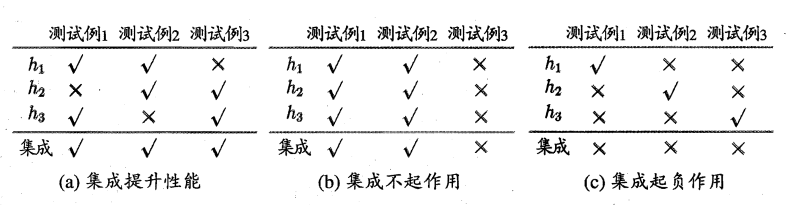
\includegraphics[width=0.8\textwidth]{../img/8-2-集成个体应“好而不同”.png}
    \caption{集成个体应“好而不同”}
    \label{fig:集成个体应“好而不同”}
\end{figure}

0


\end{document}